\section{Analysis}
\label{sec:analysis}
In the main text, we retain only analyses that directly support our core
claims, namely why SPRM benefits from additive supervision components and why
filtering is necessary for local credit assignment. Implementation-focused analyses,
including Stage 1 model selection, input feature selection, and IG baseline
selection, are deferred to Appendix~\ref{sec:appendix}.

\subsection{Ablation Study}
\label{ablation_study}
Under fixed backbone, training-data scale, and optimization hyperparameters, we
perform additive ablations over the key SPRM modules.

\todo{use table and redesign the ablation study to verify the role of each component in a more targeted manner.}
\begin{figure*}[t]
\centering
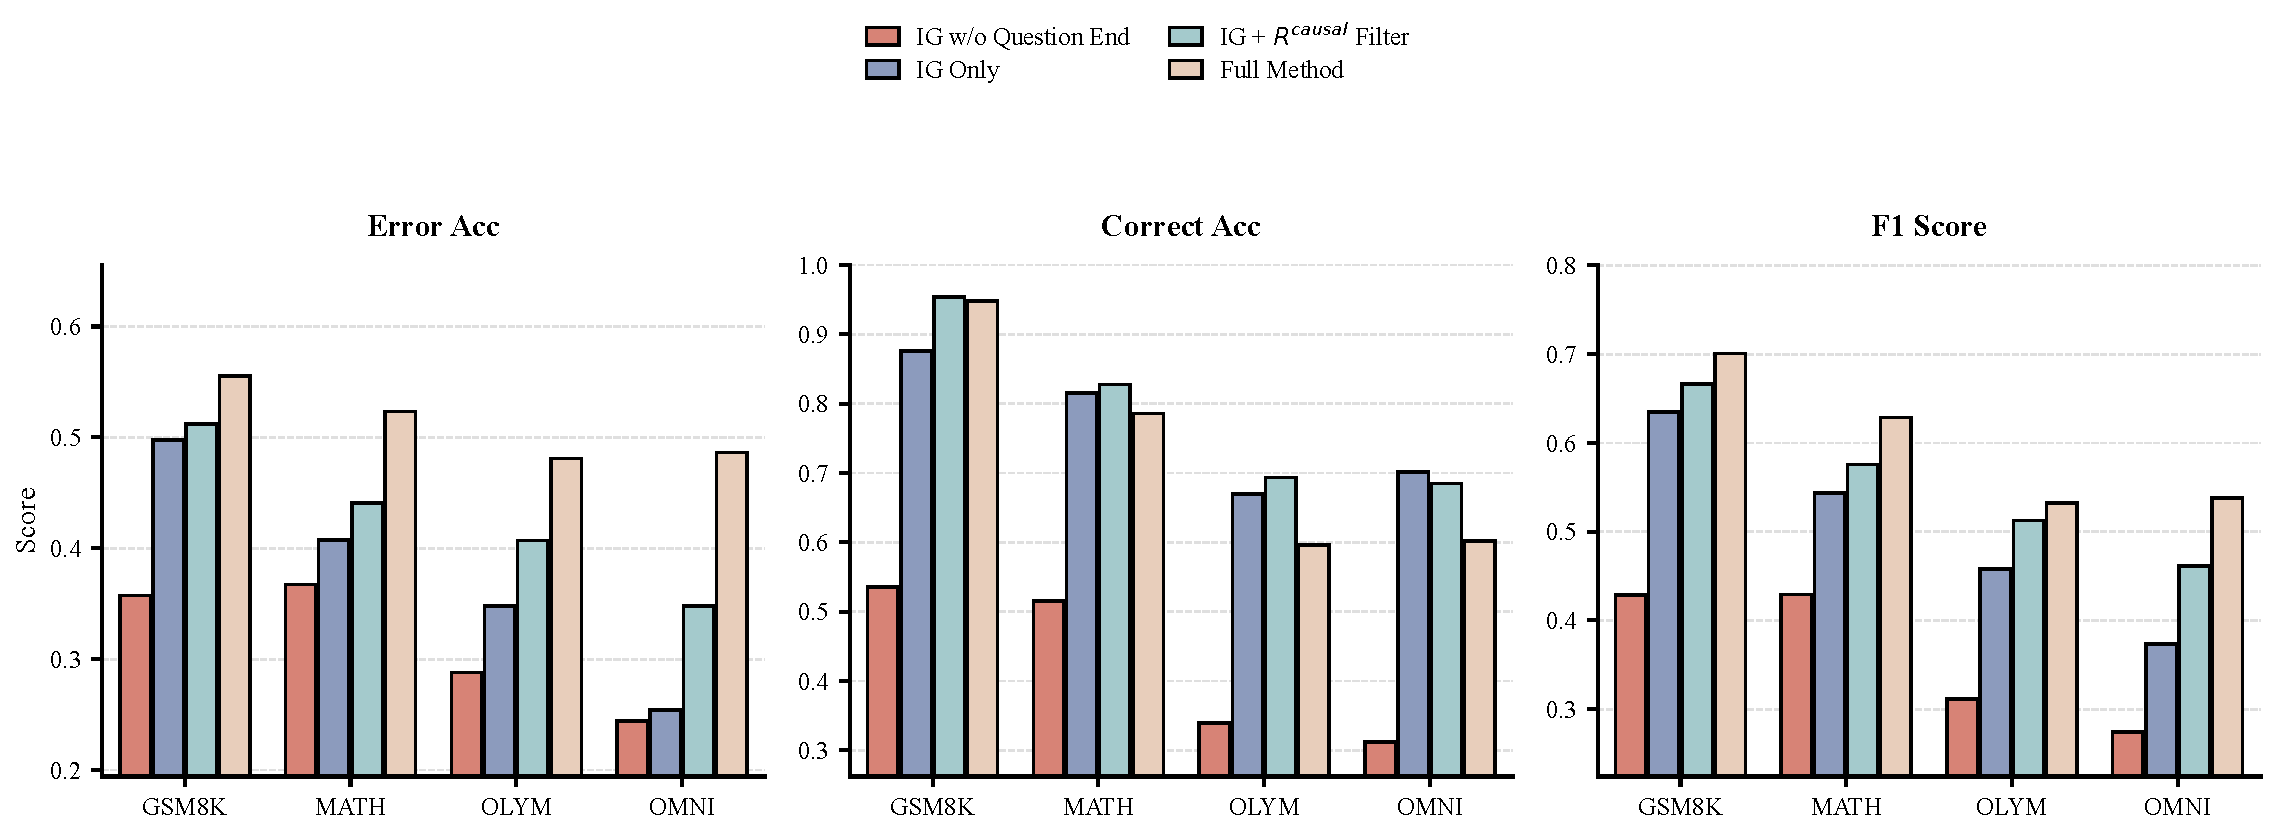
\includegraphics[width=\textwidth]{figures/ablation_all_metrics.pdf}
\caption{Ablation results of SPRM across all reported metrics. The figure
summarizes the contribution of each module under a unified
training/evaluation protocol.}
\label{fig:ablation_all_metrics}
\end{figure*}

Figure~\ref{fig:ablation_all_metrics} reports four variants under a unified
protocol:
(1) IG-only local supervision without the question-boundary state \(x_{i,0}\);
(2) IG with the question-boundary state;
(3) IG with the question-boundary state and
\(R_{i,t}^{\mathrm{causal}}\) filtering; and
(4) the full SPRM that further adds \(\delta_{\mathrm{global}}\).

Three observations are consistent across metrics.
First, introducing the question-boundary state improves boundary calibration,
showing that local attribution should not start from the first reasoning step
alone.
The transition from the problem statement to the reasoning chain already
contains information about how subsequent steps should be interpreted, so
including \(x_{i,0}\) gives the scorer a more stable anchor for the first
credit-assignment decision.
Second, adding \(R_{i,t}^{\mathrm{causal}}\) further stabilizes training and
improves the balance between \textit{Err} and \textit{Cor}, which indicates
that raw IG-based local signals contain non-trivial noise and benefit from a
dependency-aware counterfactual agreement check.
Third, incorporating \(\delta_{\mathrm{global}}\) brings the strongest gains on
the harder domains, especially OLYMPIADBENCH and OMNIMATH.
Although \textit{Cor} may slightly decrease in some settings, the overall F1
improves, yielding the best trade-off in the full model.

Overall, the ablation confirms that SPRM's gain does not come from a single
module.
The question-boundary state improves step alignment, causal filtering reduces
label noise in local supervision, and the global prior adds robustness against
context-dependent fluctuations in step value.

\subsection{Filtering Strategy Comparison}
We next ask two questions:
is filtering itself necessary for local supervision, and if so, why do we use
\(R_{i,t}^{\mathrm{causal}}\) rather than an alternative LLM-consistency
filter?
To answer them, we compare the two filtering strategies under the same
evaluation protocol.

\todo{use table}
\begin{figure*}[t]
\centering
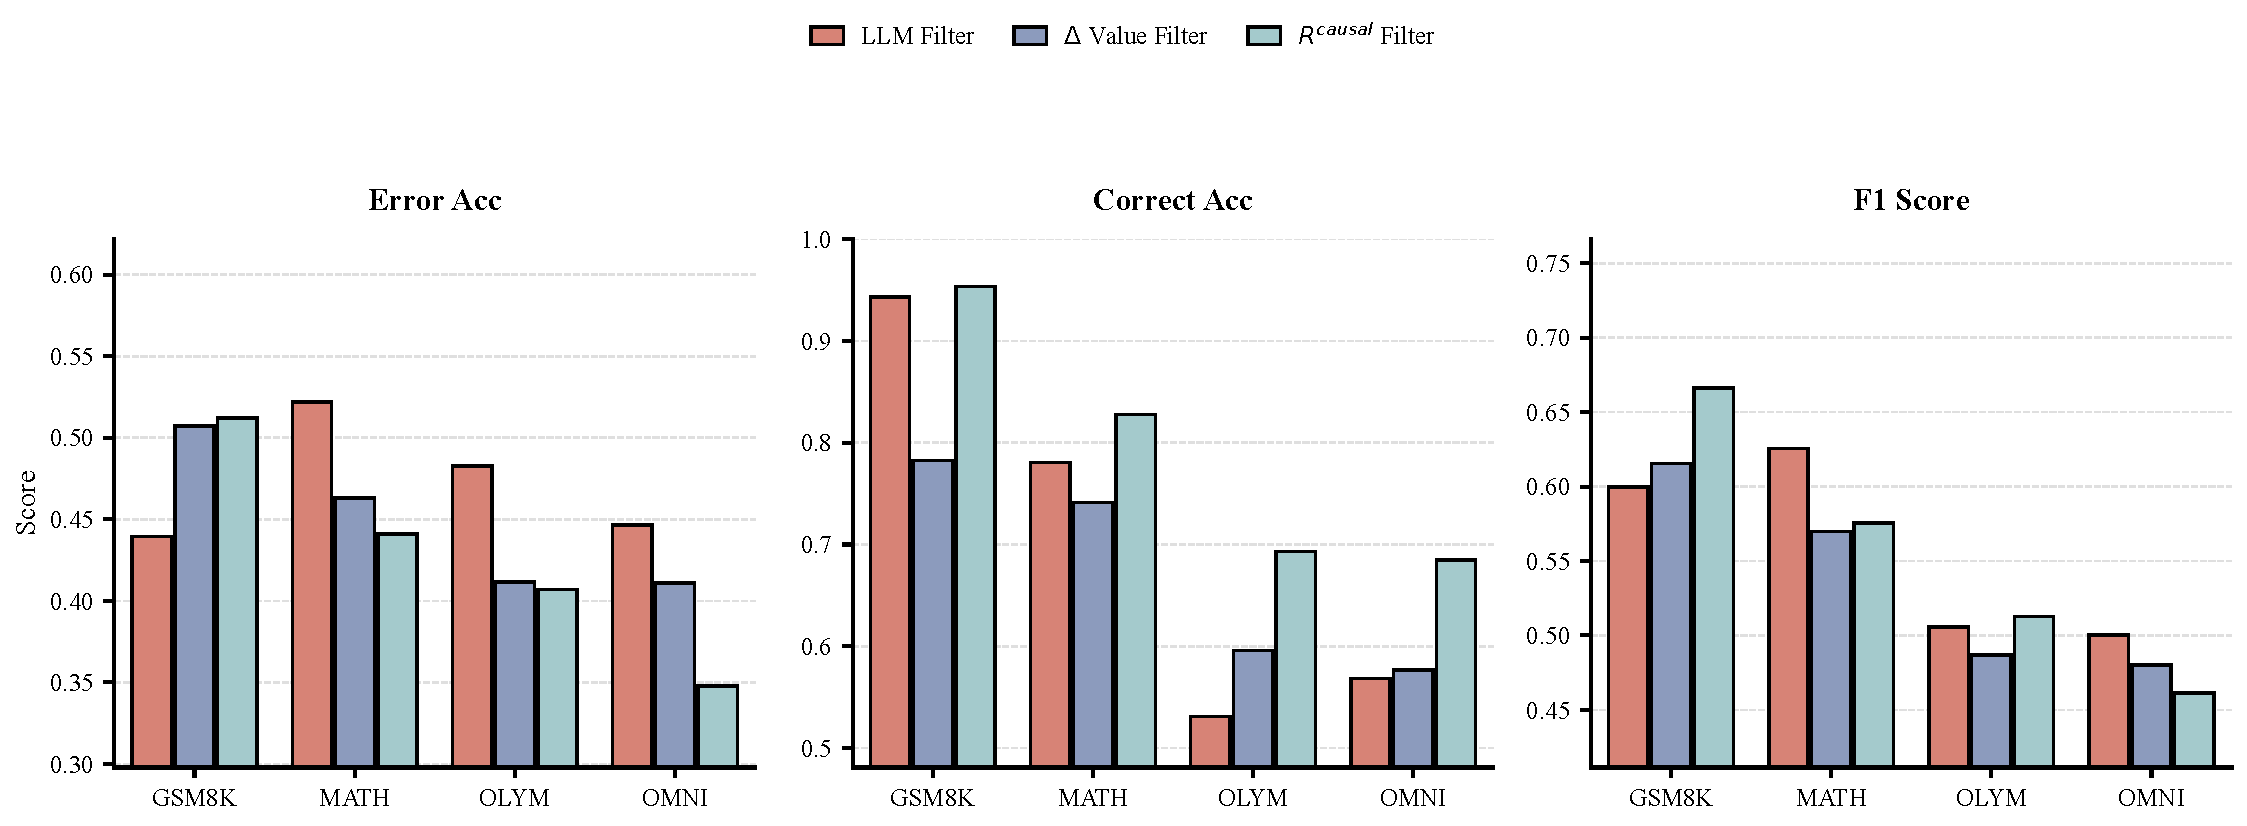
\includegraphics[width=\textwidth]{figures/filter_all_metrics.pdf}
\caption{Impact of the filtering strategy on all evaluation metrics. The plot
reports performance differences between variants with and without filtering
strategies.}
\label{fig:filter_all_metrics}
\end{figure*}

As shown in Figure~\ref{fig:filter_all_metrics}, both filters improve over
using raw local attribution alone, which shows that a filtering stage is
necessary rather than optional.
This is consistent with the role of \(\delta_{\mathrm{local}}\): it is derived
from a learned value proxy through a path-integrated attribution procedure, so
its sign can fluctuate when the scorer is imperfect or when long trajectories
amplify local noise.
Filtering therefore acts as a reliability test before the local signal is used
as supervision.

The two filters, however, emphasize different notions of reliability.
The LLM-consistency filter is more aligned with semantic agreement and can
sharpen sensitivity-oriented indicators such as first-error localization.
By contrast, \(R_{i,t}^{\mathrm{causal}}\) directly asks whether removing the
current step remains supportive after accounting for its local interactions
with nearby preceding steps, so it is more tightly aligned with the
contextual contribution that the local head is intended to capture.
This leads to more stable gains on correct-path acceptance and stronger
behavior on the harder long-horizon benchmarks.

This comparison clarifies why the final method uses
\(R_{i,t}^{\mathrm{causal}}\).
The LLM-consistency filter is a useful empirical reference because it confirms
that denoising local credit matters, but the counterfactual filter is more
faithful to our target quantity: whether the current step helps or hurts the
outcome of the specific trajectory in which it appears after accounting for
its immediate step dependencies.